% !TeX program = xelatex
% !BIB program = biber
\documentclass[light]{lutbeamer}

\usepackage{pgfpages}
\usepackage{ragged2e}
\usepackage{booktabs}
\usepackage{amssymb}
\usepackage{fontawesome5}
\usepackage{tikz}
\usepackage{pgfplots}
\pgfplotsset{compat=1.18}
\addbibresource{references.bib}

% ===================================================================
% METADATA
% ===================================================================
\setdepartment{OSTIM Teknik Üniversitesi}
\institute{}
\author[Mühendislik Fakültesi]{\\Prof.~Dr.~Yalçın ATA,\\ 
Prof.~Dr.~Arif DEMİR,\\ Dr.~Öğr.~Üyesi~Emel GÜVEN,\\ Dr.~Öğr.~Üyesi~Ufuk ASIL,\\ Dr.~Öğr.~Üyesi~Haydar KILIÇ,\\ Dr.~Öğr.~Üyesi~Muhammed ELMNEFİ,\\ Öğr.~Gör.~Sema ÇİFTÇİ}
\title{MATH 204 -- Olasılık ve İstatistik}
\subtitle{Hafta 4: Rastgele Değişkenler ve Olasılık Dağılımları}
\date{2025--2026 Bahar Dönemi}

% ===================================================================
% OTOMATİK İÇİNDEKİLER
% ===================================================================
\setcounter{tocdepth}{2}

\AtBeginSection[]{
  \begin{frame}{Sunum Planı}
    \scriptsize
    \begin{columns}[T]
      \begin{column}{0.48\textwidth}
        \tableofcontents[sections={1-3}, currentsection]
      \end{column}
      \begin{column}{0.48\textwidth}
        \tableofcontents[sections={4-10}, currentsection]
      \end{column}
    \end{columns}
  \end{frame}
}

\begin{document}

\setbeamertemplate{navigation symbols}{}
\setbeamertemplate{footline}{
  \begin{beamercolorbox}[wd=\paperwidth, ht=10pt, dp=1pt]{footline}
    \usebeamerfont{footline}
    \begin{tikzpicture}[remember picture,overlay]
      \node[anchor=south west, xshift=10mm, yshift=.4mm]
      at (current page.south west)
      {\insertshortauthor,~\department};
    \end{tikzpicture}
    \begin{tikzpicture}[remember picture,overlay]
      \node[anchor=south east, xshift=-5mm, yshift=0.5mm]
      at (current page.south east)
      {\insertframenumber \,/\, \inserttotalframenumber};
    \end{tikzpicture}
  \end{beamercolorbox}
}

% ===================================================================
% KAPAK
% ===================================================================
\begin{frame}<article:0>[plain,noframenumbering]
  \begin{tikzpicture}[remember picture,overlay]
    \node[anchor=center, at=(current page.center), inner sep=0pt] {
      \includegraphics[width=\paperwidth, height=\paperheight]{logos/background_figure.jpg}
    };
  \end{tikzpicture}
\end{frame}

{
  \setbeamertemplate{footline}{
    \begin{beamercolorbox}[wd=\paperwidth, ht=10pt, dp=1pt]{footline}
      \usebeamerfont{footline}
      \begin{tikzpicture}[remember picture,overlay]
        \node[anchor=south west, xshift=10mm, yshift=.4mm, align=left]
        at (current page.south west)
        {\tiny Bu şablon OTU Yazılım Mühendisliği tarafından hazırlanmış olup \href{https://github.com/ufukasia/Ostim-Teknik--niversitesi-Yaz-l-m-M-hendisli-i---Lutbeamer-egitim-i-eri-i-haz-rlama-}{buradan} güncel haline ulaşabilirsiniz.};
      \end{tikzpicture}
      \begin{tikzpicture}[remember picture,overlay]
        \node[anchor=south east, xshift=-5mm, yshift=0.5mm]
        at (current page.south east)
        {\insertframenumber \,/\, \inserttotalframenumber};
      \end{tikzpicture}
    \end{beamercolorbox}
  }
  \maketitle{}
}

% İÇİNDEKİLER
\begin{frame}{İçindekiler}
  \scriptsize
  \begin{columns}[T]
    \begin{column}{0.48\textwidth}
      \tableofcontents[sections={1-3}]
    \end{column}
    \begin{column}{0.48\textwidth}
      \tableofcontents[sections={4-10}]
    \end{column}
  \end{columns}
\end{frame}




\begin{frame}{Hafta 3'ten Ne Getiriyoruz?}
    \begin{block}{Temel Hatırlatma}
        Geçen hafta öğrendiğimiz araçlar:
        \[
        P(A|B)=\frac{P(A\cap B)}{P(B)}, \qquad
        P(A)=\sum_{i}P(B_i)P(A|B_i), \qquad
        P(B_r|A)=\frac{P(B_r)P(A|B_r)}{P(A)}.
        \]
    \end{block}

    \begin{itemize}
        \item Bağımsızlık, Toplam Olasılık ve Bayes ile olayların olasılıklarını hesapladık.
        \item Ama hep \textbf{olaylar} (``bozuk çıktı'', ``makine~1'den geldi'') ile uğraştık.
        \item \textbf{Bu hafta:} Sonuçları \textbf{sayıya çevirme} -- Rastgele Değişkenler.
    \end{itemize}
\end{frame}




% ===================================================================
% KAVRAM HARITASI - KENDI KENDINE CALISMAYA UYGUN ACIKLAMALI
% ===================================================================
\begin{frame}{Kavram Haritası: Rastgele Değişkenler Nerede?}
    \vspace{0.2cm}
    \centering
    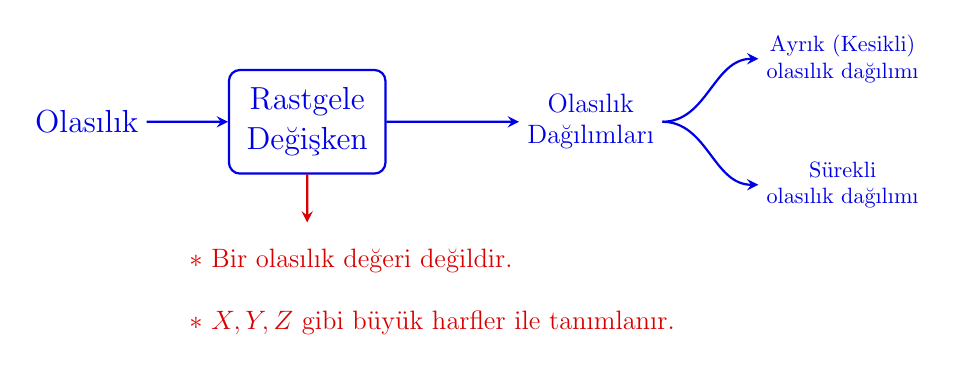
\begin{tikzpicture}[scale=0.80, transform shape, >=stealth, thick]

        % MAVI KALEM KISMI
        \node[text=blue!90!black, font=\Large] (olasilik) at (-4.5, 2) {Olasılık};
        \node[draw=blue!90!black, rounded corners, inner sep=8pt, text=blue!90!black, font=\Large, align=center] (rastgele) at (-1, 2) {Rastgele\\Değişken};
        \node[text=blue!90!black, font=\large, align=center] (dagilim) at (3.5, 2) {Olasılık\\Dağılımları};

        \node[text=blue!90!black, font=\normalsize, align=center] (ayrik_dag) at (7.5, 3) {Ayrık (Kesikli)\\olasılık dağılımı};
        \node[text=blue!90!black, font=\normalsize, align=center] (surekli_dag) at (7.5, 1) {Sürekli\\olasılık dağılımı};

        % Mavi Oklar
        \draw[->, blue!90!black] (olasilik) -- (rastgele);
        \draw[->, blue!90!black] (rastgele) -- (dagilim);
        \draw[->, blue!90!black] (dagilim.east) to[out=0, in=180] (ayrik_dag.west);
        \draw[->, blue!90!black] (dagilim.east) to[out=0, in=180] (surekli_dag.west);

        % KIRMIZI/PEMBE KALEM KISMI
        \colorlet{mypink}{red!85!black}
        \node[text=mypink, font=\large, align=left, anchor=west] (prop1) at (-3, -0.2) {\textbf{$\ast$} Bir olasılık değeri değildir.};
        \node[text=mypink, font=\large, align=left, anchor=west] (prop2) at (-3, -1.2) {\textbf{$\ast$} $X, Y, Z$ gibi büyük harfler ile tanımlanır.};
        \draw[->, mypink] (rastgele.south) -- (-1, 0.4);
    \end{tikzpicture}

    \vspace{0.2cm}
    \begin{exampleblock}{Önemli Kılavuz Bilgi}
        \footnotesize Rastgele değişken tek başına bir olasılık sonucu (\%50, 0.2 vb.) \textbf{değildir}. Olasılık deneyindeki fiziksel durumları (zar atma, para atma), sayılara dökerek \textbf{istatistiğe geçişi sağlayan bir köprüdür}.
    \end{exampleblock}
\end{frame}

% ===================================================================
% AYRIK RASTGELE DEGISKENIN DOGASI - ETKILESIMLI/ADIM ADIM COZUM
% ===================================================================
\begin{frame}[t]{Ayrık Rastgele Değişkenin Doğası}
    \normalsize
    \textbf{\textcolor{blue!80!black}{\underline{Ayrık Rastgele Değişken}:}} Bir şeylerin sayısıdır. \\
    \small \textcolor{gray}{\textit{(the number of \dots)}}
    
    \vspace{0.1cm}
    \centering
    \begin{tikzpicture}[>=stealth, thick, scale=0.62, transform shape]
        \colorlet{myblue}{blue!80!black}

        % BIRINCI ORNEK (TAMAMLANMIS SUREC)
        \node[draw=myblue, rounded corners=15pt, minimum width=3.5cm, minimum height=1.5cm, align=center, text=myblue] (deney1) at (0, 0) {Bir para 3 kez\\atılıyor.};
        \node[text=myblue, font=\footnotesize] at (0, -1.1) {Olasılık deneyi};

        \node[draw=myblue, rounded corners=5pt, minimum width=4cm, minimum height=2cm, align=center, text=myblue] (degisken1) at (5, 0) {$X$: tura gelmelerinin\\sayısı\\[0.3cm] $X = \{0, 1, 2, 3\}$};

        \node[text=myblue] (tablo1) at (10.5, 0) {
            \renewcommand{\arraystretch}{1.5}
            \begin{tabular}{c|cccc}
                $X$ & 0 & 1 & 2 & 3 \\
                \hline
                $P(X=x)$ & & & & 
            \end{tabular}
        };

        \draw[->, myblue] (deney1.east) -- (degisken1.west);
        \draw[->, myblue] (degisken1.east) -- (tablo1.west);

        % IKINCI ORNEK (ZAR ATMA)
        \node[draw=myblue, rounded corners=15pt, minimum width=3.5cm, minimum height=1.5cm, align=center, text=myblue] (deney2) at (0, -3.5) {Bir zar 2 kez\\atılıyor.};
        \node[text=myblue, font=\footnotesize] at (0, -4.6) {Olasılık deneyi};

        % OVERLAY: O grenci ilk basta sadece soruyu gorur, sonraki tiklamada cozumu gorur.
        \only<1>{
            \node[align=left, text=myblue, font=\Large] (degisken2_soru) at (4.5, -3.5) {$Y$ : \dots\dots\dots\dots\dots ?};
            \draw[->, myblue] (deney2.east) -- (4, -3.5);
        }
        
        \only<2->{
            \node[draw=red!80!black, rounded corners=5pt, minimum width=4cm, minimum height=2cm, align=center, text=red!80!black] (degisken2_cevap) at (5, -3.5) {$Y$: \textbf{5} gelmelerinin\\sayısı\\[0.3cm] $Y = \{0, 1, 2\}$};
            \draw[->, myblue] (deney2.east) -- (degisken2_cevap.west);
        }

    \end{tikzpicture}

    \vspace{0.05cm}
    \footnotesize
    \only<1>{
        \begin{alertblock}{Kendi Kendine Düşünme Adımı}
            İkinci örnekte para yerine zar atıyoruz. $Y$ ayrık rastgele değişkenini siz tanımlayacak olsaydınız cümleyi nasıl kurardınız? \textbf{Alabileceği değerler kümesi ($Y = \{ \dots \}$) ne olurdu?}
        \end{alertblock}
    }
\end{frame}

\begin{frame}{Çözüm: Zar Örneğinde Ayrık Değişkenin Değerleri}
    \small
    \begin{columns}[T]
        \begin{column}{0.52\textwidth}
            \begin{block}{Tanım}
                \[
                Y = \text{2 atışta gelen 5 sayısı}
                \]
            \end{block}

            \begin{block}{Değer Kümesi Neden \(\{0,1,2\}\)?}
                \begin{itemize}
                    \item Hiç 5 gelmezse: \(Y=0\)
                    \item Tam bir kez 5 gelirse: \(Y=1\)
                    \item İki kez de 5 gelirse: \(Y=2\)
                \end{itemize}
            \end{block}

            \begin{alertblock}{Bağlantı}
                Bu küme, ayrık rastgele değişkenin alabileceği tüm sayısal sonuçları verir. Bir sonraki adım: her değerin olasılığını yazıp dağılımı kurmak.
            \end{alertblock}
        \end{column}
        \begin{column}{0.46\textwidth}
            \centering
            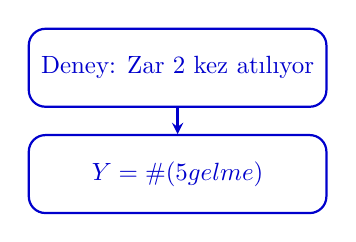
\begin{tikzpicture}[>=stealth, scale=0.9, transform shape, thick]
                \colorlet{myblue}{blue!80!black}

                \node[draw=myblue, rounded corners=6pt, align=center, minimum width=4.2cm, minimum height=1.1cm, text=myblue] (exp) at (0,2.1) {Deney: Zar 2 kez atılıyor};
                \node[draw=myblue, rounded corners=6pt, align=center, minimum width=4.2cm, minimum height=1.1cm, text=myblue] (var) at (0,0.6) {$Y=\#(\text{5 gelme})$};
                \draw[->, myblue] (exp) -- (var);
            \end{tikzpicture}

            \vspace{0.2cm}
            \begin{tabular}{c|c}
                Durum & \(Y\) \\
                \hline
                \(5\) yok & 0 \\
                bir tane \(5\) & 1 \\
                iki tane \(5\) & 2 \\
            \end{tabular}

            \vspace{0.2cm}
            \[
            Y \in \{0,1,2\}
            \]
        \end{column}
    \end{columns}
\end{frame}

% ===================================================================
% BÖLÜM 1: KÖPRÜ + MOTİVASYON
% ===================================================================

\begin{frame}{Motivasyon: Neden Sayılara İhtiyacımız Var?}
\footnotesize
\begin{columns}[T]
  \begin{column}{0.55\textwidth}
    \begin{block}{Senaryo Açıklaması}
      Pek çok durumda olayların sonuçlarını doğrudan analiz etmek zordur. Örneğin 3 elektronik bileşenin test sonuçlarını (S: Sağlam, A: Arızalı) düşünelim:
      \[
      S = \{SSS, SSA, SAS, ASS, SAA, ASA, AAS, AAA\}
      \]
      Bu 8 durum üzerinden işlem yapmak karmaşıktır.
    \end{block}

    \begin{block}{Çözüm: Sayısal Özet Çıkarmak}
      Bunun yerine sadece ``\textbf{Kaç tane arızalı bileşen var?}'' sorusuna odaklanalım:
      \[
      X = \text{arızalı bileşen sayısı}
      \] 
    \end{block}
  \end{column}
  \begin{column}{0.42\textwidth}
    \centering
    \textbf{Dönüşüm Tablosu ($X$ Eşlemesi)}
    \vspace{0.15cm}
    
    \begin{tabular}{c c c}
      \toprule
      Harfli Durum & $\xrightarrow{X}$ & Arızalı Sayısı ($x$) \\
      \midrule
      $SSS$ & $\rightarrow$ & \textbf{0} \\
      $SSA, SAS, ASS$ & $\rightarrow$ & \textbf{1} \\
      $SAA, ASA, AAS$ & $\rightarrow$ & \textbf{2} \\
      $AAA$ & $\rightarrow$ & \textbf{3} \\
      \bottomrule
    \end{tabular}
    
    \vspace{0.4cm}
    \begin{alertblock}{Ana Fikir Niye Önemli?}
      X dediğimiz bu kavram, o 8 durumu alır ve sadece $X \in \{0, 1, 2, 3\}$ gibi 4 tane basit sayıyla ifade etmemizi sağlar.
    \end{alertblock}
  \end{column}
\end{columns}
\end{frame}

% ===================================================================
% BÖLÜM 2: RASTGELE DEĞİŞKEN KAVRAMI (Kitap 3.1)
% ===================================================================
\section{Rastgele Değişken Kavramı (Bölüm 3.1)}
\subsection{Tanım ve Temel Örnekler}

\begin{frame}{Kavrama Giriş: Rastgele Değişken Nedir? (Tanım 3.1)}
    \begin{block}{Tanım (Kitap, Definition 3.1)}
        Rastgele değişken, örnek uzaydaki \textbf{her elemana bir reel sayı atayan} fonksiyondur:
        \[
        X : S \to \mathbb{R}, \qquad \omega \mapsto X(\omega).
        \]
    \end{block}

    \begin{itemize}
        \item $X$: Rastgele değişkenin adı (büyük harf).
        \item $x$: $X$'in alabileceği belirli bir değer (küçük harf).
        \item $\{X = x\}$: ``$X$'in $x$ değerini aldığı'' olay; bu, $S$'nin bir alt kümesidir.
    \end{itemize}

    \begin{exampleblock}{Basit Analoji}
      Sınavda öğrenciler farklı cevaplar verir ($\omega$); not fonksiyonu ($X$) her cevap kâğıdına bir puan atar.
    \end{exampleblock}
\end{frame}

\begin{frame}{Örnek Uzayların Sınıflandırılması: Ayrık Örnek Uzay}
    \begin{block}{Tanım (Kitap, Definition 3.2): Ayrık Örnek Uzay}
        Eğer bir örnek uzay, sonlu sayıda olasılık barındırıyorsa ya da tamsayılar kümesi kadar elemanı olan sonsuz bir dizi içeriyorsa, buna \textbf{ayrık örnek uzay} denir.
    \end{block}

    \begin{exampleblock}{Sürekli Örnek Uzaylara Neden İhtiyaç Duyarız?}
        Bazı istatistiksel deneylerin sonuçları sonlu ya da sayılabilir olmayabilir:
        \begin{itemize}
            \item Belirli marka bir otomobilin 5~litre benzinle test parkurunda kat edeceği mesafenin ölçülmesi. Mesafenin istenilen her hassasiyette ölçülebildiği varsayılırsa, tamsayılarla eşleştirilemeyecek kadar sonsuz sayıda olası mesafe vardır.
            \item Bir kimyasal tepkimenin gerçekleşme süresinin kaydedilmesi. Örnek uzayımızı oluşturan olası zaman aralıkları sayılamayacak kadar çok ve sonsuz sayıda olurdu.
        \end{itemize}
        Tüm örnek uzayların ayrık olması gerekmez.
    \end{exampleblock}
\end{frame}

\begin{frame}{Sürekli Örnek Uzay ve Rastgele Değişken Türleri}
    \begin{block}{Tanım (Kitap, Definition 3.3): Sürekli Örnek Uzay}
        Eğer bir örnek uzay, bir doğru parçası üzerindeki noktaların sayısına eşit olacak kadar sonsuz sayıda olasılık içeriyorsa, buna \textbf{sürekli örnek uzay} denir.
    \end{block}

    \begin{block}{Ayrık ve Sürekli Rastgele Değişkenler}
        \begin{itemize}
            \item \textbf{Ayrık Rastgele Değişken:} Eğer rastgele bir değişkenin alabileceği sonuçlar kümesi sayılabilir ise, buna ayrık rastgele değişken denir. (Önümüzdeki Örnek~3.1--3.5 kapsamındaki değişkenler ayrıktır.)
            \item \textbf{Sürekli Rastgele Değişken:} Alabileceği değerler kümesi sayı doğrusu üzerinde tam bir aralık olan rastgele değişken ayrık değildir, \textbf{sürekli rastgele değişkendir}.
        \end{itemize}
    \end{block}
\end{frame}

\begin{frame}{Soyuttan Somuta: Torbadan Top Çekme Macerası (Örnek 3.1)}
\footnotesize
\begin{columns}[T]
  \begin{column}{0.55\textwidth}
    \begin{block}{Problem}
      Bir torbada 4 kırmızı, 3 siyah top var. Yerine koymadan 2 top çekiliyor.
      $Y$: çekilen \textbf{kırmızı top sayısı}.
    \end{block}

    \begin{alertblock}{Çözüm}
      Y rastgele değişkenin $y$ değerleri bu şekilde yazılır:
      \vspace{0.15cm}\\
      \centering
      \begin{tabular}{cc}
        \toprule
        Sonuç & $Y$ değeri \\
        \midrule
        $KK$ & 2 \\
        $KS$ & 1 \\
        $SK$ & 1 \\
        $SS$ & 0 \\
        \bottomrule
      \end{tabular}
    \end{alertblock}
  \end{column}
  \begin{column}{0.42\textwidth}
    \begin{block}{Önemli Gözlem}
      \begin{itemize}
        \item $KS$ ve $SK$ farklı sonuçlar ama ikisi de $Y=1$ verir.
        \item Eşleme \textbf{çoktan-bire} olabilir.
        \item $\{Y=1\} = \{KS, SK\}$ bir olaydır.
      \end{itemize}
    \end{block}
  \end{column}
\end{columns}
\end{frame}

\begin{frame}{İmkansız Değerleri Fark Etmek: Baret Eşleştirme (Örnek 3.2)}
\footnotesize
\vspace{-1cm}
\begin{columns}[T]
  \begin{column}{0.54\textwidth}
    \begin{block}{Senaryonun Özü}
      \textbf{Ahmet (A), Berk (B) ve Can (C)}'nin baretleri karıştırılıyor ve rastgele geri dağıtılıyor. Meydana gelebilecek \textbf{toplam $3! = 6$ farklı olasılık} vardır.
      Rastgele değişkenimiz:
      \[
      E = \text{kendi baretini doğru alan işçi sayısı}
      \]
    \end{block}

    \vspace{0.05cm}
    \scriptsize
    Not: Tablodaki örneğin \textbf{ACB} dizilimi $\rightarrow$ Ahmet'in \textbf{A}'yı, Berk'in \textbf{C}'yi, Can'ın \textbf{B}'yi alması durumunu temsil eder.

    \centering
    \begin{tabular}{lc}
      \toprule
      Tüm Olası Dağıtım Durumları ($\omega$) & Rastgele Değişken ($E$) \\
      \midrule
      $ABC$ (Herkes doğru) & 3 \\
      $ACB$ (Sadece Ahmet doğru) & 1 \\
      $BCA$ (Kimse doğru alamadı) & 0 \\
      $CAB$ (Kimse doğru alamadı) & 0 \\
      $CBA$ (Sadece Can doğru) & 1 \\
      $BAC$ (Sadece Berk doğru) & 1 \\
      \bottomrule
    \end{tabular}
  \end{column}
  \vspace{-1cm}
  \begin{column}{0.44\textwidth}
    \begin{block}{Olayların Sayısal Kümelenmesi}
      Rastgele değişken ($E$) tüm kalabalık senaryoları aldı ve sadece 3 kümeye indirdi:
      \begin{itemize}
        \item \textbf{Hiçbiri Alamayanlar:} \\ $\{E=0\} = \{BCA, CAB\}$
        \item \textbf{Sadece 1 Kişi Alanlar:} \\ $\{E=1\} = \{ACB, CBA, BAC\}$
        \item \textbf{Herkesin Doğru Aldığı:} \\ $\{E=3\} = \{ABC\}$
      \end{itemize}
    \end{block}
    \begin{alertblock}{Mantıksal Çıkarım: Neden "E=2" Yok?}
      Rastgele değişken $E$'nin alabileceği değerler arasında $E=2$ \textbf{imkansızdır}! 
      Çünkü 3 kişiden \textbf{ikisi} doğru bareti aldıysa, mecburen geriye kalan son kişi de kendi baretini almış demektir (Bu durumda $E$ otomatikman 3 olur).
    \end{alertblock}
  \end{column}
\end{columns}
\end{frame}

\begin{frame}{Sadece ``Evet'' veya ``Hayır'' Diyen Değişken (Örnek 3.3)}
\begin{block}{Problem}
  Üretim hattından gelen bileşenler sağlam ($S$) veya arızalı ($A$) olabiliyor.
  Bu durumu sayıya çevirmek istiyoruz.
\end{block}

\[
X =
\begin{cases}
1, & \text{bileşen arızalı ise},\\
0, & \text{bileşen sağlam ise}.
\end{cases}
\]

\begin{block}{Yorum}
  \begin{itemize}
    \item 0 ve 1 ataması keyfidir ama çok kullanışlıdır.
    \item Bu tür iki değerli değişken yapıları istatistikte temel bir yapıtaşıdır.
    \item İleride (Bölüm 5) bu yapıyı çok kullanacağız.
  \end{itemize}
\end{block}
\end{frame}

\begin{frame}{Örnek 3.5: Ufku Genişletmek, Sayılabilir Sonsuzluk}
\small
Bir üretim bandından arızalı ($A$) bir ürün gelene kadar parça seçiliyor. Sağlam ürünler $S$ ile gösterilir.
\begin{center}
\begin{tabular}{llc}
    \toprule
    Örnek Nokta ($\omega$) & Açıklama & $X$ \\
    \midrule
    $A$ & İlk parça arızalı & 1 \\
    $SA$ & İkinci parça arızalı & 2 \\
    $SSA$ & Üçüncü parça arızalı & 3 \\
    $SSSA$ & Dördüncü parça arızalı & 4 \\
    $\vdots$ & $\vdots$ & $\vdots$ \\
    \bottomrule
\end{tabular}
\end{center}
\begin{alertblock}{Önemli Gözlem}
    $X \in \{1, 2, 3, \dots\}$: Değer kümesi \textbf{sayılabilir sonsuz}dur. Bu da ayrık bir rastgele değişkendir.
\end{alertblock}
\end{frame}

\begin{frame}{Kritik Eşik: Sonsuz Sayıda Olmak ``Sürekli'' Demek Midir?}
\small
\begin{block}{Asıl Mesaj}
Bu örnek, \textbf{ayrık} demek için sadece ``sonlu değer'' gerekmediğini öğretir.
\textbf{Sonsuz sayıda değer} olsa bile, değerler numaralanabiliyorsa (\(1,2,3,\dots\)) değişken yine ayrık kalır.
\end{block}

\begin{columns}[T]
  \begin{column}{0.58\textwidth}
    \begin{alertblock}{Pratik Kazanım}
      \begin{itemize}
        \item ``İlk başarıya kadar deneme sayısı'' türündeki problemleri tanırsın.
        \item Böyle durumlarda değer kümesini doğru kurarsın: \(X\in\{1,2,3,\dots\}\).
        \item PMF yazarken sonsuz toplamla çalışman gerektiğini erken görürsün.
      \end{itemize}
    \end{alertblock}
  \end{column}
  \begin{column}{0.38\textwidth}
    \begin{block}{Devam Bağlantısı}
      Bir sonraki adımda bu fikir, ``ayrık vs sürekli'' ayrımını netleştirir:
      \[
      \text{sayılabilir} \Rightarrow \text{ayrık}
      \]
      \[
      \text{aralık tipi} \Rightarrow \text{sürekli}
      \]
    \end{block}
  \end{column}
\end{columns}
\end{frame}
\subsection{Ayrık ve Sürekli Rastgele Değişken Ayrımı}

\begin{frame}{Adım 1: Sadece Sayabildiklerimiz (Ayrık/Kesikli Değişken Olgusu)}
\begin{block}{Hatırlatma (Tanım 3.2): Ayrık Örnek Uzay}
  Bir deneyin tüm olası sonuçları \textbf{sonlu} veya \textbf{sayılabilir sonsuz} sayıda (1, 2, 3, \dots) eleman içeriyorsa, bu yapıya \textbf{ayrık} denir. Burada sayılar arasına adım adım gidilir.
\end{block}

\begin{columns}[T]
  \begin{column}{0.55\textwidth}
    \begin{exampleblock}{Kitap Örnekleri}
      \begin{itemize}
        \item \textbf{Ex 3.4:} 100'lük partiden 10 ürün seçiliyor. $X$: arızalı sayısı.
        $X \in \{0, 1, 2, \dots, 10\}$ -- \textbf{sonlu}.
        \item \textbf{Ex 3.5:} Üretim bandında arızalı bir ürün çıkana kadar ürün kontrol ediliyor.\\
        $X \in \{1, 2, 3, \dots\}$ -- \textbf{sayılabilir sonsuz}.
      \end{itemize}
    \end{exampleblock}
  \end{column}
  \begin{column}{0.42\textwidth}
    \begin{alertblock}{Ayrık Olma Ölçütü}
      Değer kümesi \textbf{sayılabilir} ise (sonlu veya $1, 2, 3, \dots$ gibi numaralanabilir) değişken \textbf{ayrık}tır.
    \end{alertblock}
  \end{column}
\end{columns}
\end{frame}

\begin{frame}{Adım 2: Ölçebildiklerimiz ve Aralıklar (Sürekli Değişken Olgusu)}
\begin{block}{Hatırlatma (Tanım 3.3): Sürekli Örnek Uzay}
  Deneyin sonuçları bir doğru parçası (veya ölçüm aralığı) üzerindeki \textbf{tüm noktaları} (sayısız ondalıklı değeri) içeriyorsa kesintisiz bir akış vardır ve buna \textbf{sürekli} denir.
\end{block}

\begin{columns}[T]
  \begin{column}{0.55\textwidth}
    \begin{exampleblock}{Kitap Örnekleri}
      \begin{itemize}
        \item \textbf{Ex 3.6:} Posta yanıt oranı. $X \in [0, 1]$.
        \item \textbf{Ex 3.7:} İki ihlal arası bekleme süresi. $X \in [0, \infty)$.
      \end{itemize}
    \end{exampleblock}
  \end{column}
  \begin{column}{0.42\textwidth}
    \begin{alertblock}{Kritik Fark}
      Sürekli değişkende \textbf{tek nokta} olasılığı \textbf{sıfırdır}:
      $P(X = 164) = 0$.

      Olasılık \textbf{aralıklardan} hesaplanır:
      $P(163 < X < 165)$.
    \end{alertblock}
  \end{column}
\end{columns}
\end{frame}

\begin{frame}{Uygulama: Posta Yanıt Oranı (Örnek 3.6)}
\small
\begin{block}{Soru}
  Bir şirket, ürettiği yeni ürünün tanıtımı için binlerce kişiye e-posta gönderiyor. 
  Şirket, bu e-postalara tıklayıp \textbf{geri dönüş yapan insanların oranını} ölçmek istiyor. 
  $X$ rastgele değişkeni, geri dönüş yapanların toplam sayısının gönderilen e-posta sayısına oranı olsun.
  $X$'in alabileceği değer aralığını ve değişkenin türünü belirleyiniz.
\end{block}

\begin{alertblock}{Çözüm ve Karar}
  \textbf{1. Değer Aralığının Tespiti:} \\
  Bir "oran", her zaman en az 0 (hiç kimse dönmedi) ve en çok 1 (herkes döndü) olabilir.
  Yani $X$ değeri 0 ile 1 arasındaki \textbf{tüm tam ve ondalıklı sayıları} ($0.12$, $0.4578$, $\dots$) alabilir.
  \vspace{0.15cm}
  
  \textbf{2. Değişkenin Türü:} \\
  Bu değerler $1, 2, 3$ şeklinde sayılamaz, bir sayı doğrusu üzerindeki bütün noktaları içeren tam bir kesittir.
  
  \textbf{Sonuç:} $X \in [0, 1]$ aralığında değer alan \textbf{Sürekli Rastgele Değişken}'dir.
\end{alertblock}
\end{frame}

\begin{frame}{Uygulama: Radar Kontrolünde Bekleme (Örnek 3.7)}
\small
\begin{columns}[T]
  \begin{column}{0.55\textwidth}
    \begin{block}{Soru}
      Bir otoyolun kenarına yerleştirilmiş radar cihazı var. 
      Cihaz ilk aşırı hız yapan aracı yakaladıktan sonra, \textbf{bir sonraki hız ihlali yapan araca kadar geçen bekleme süresini (saat cinsinden)} kronometre ile ölçüyor.
      Bu süreyi $X$ değişkeni ile tanımlarsak, $X$'in uzay kümesi ve yapısı nasıldır?
    \end{block}
  \end{column}
  
  \begin{column}{0.42\textwidth}
    \begin{alertblock}{Çözüm ve Karar}
      \textbf{Zamanın Doğası:} \\
      İki olay arasındaki geçen süre "sayılan" bir adet değil, "ölçülen" bir olgudur. 
      Bekleme süresi 1 saat, 1.5 saat veya $1.0003$ saat olabilir. Sonsuz bir bölünebilme vardır.
      
      \vspace{0.15cm}
      \textbf{Kısıtlar:} \\
      Geçen zaman negatif olamaz ($X \ge 0$). Teorik olarak bir sonraki ihlalin ne zaman olacağının bir üst sınırı da yoktur.
      
      \vspace{0.15cm}
      \textbf{Sonuç:} $X \in [0, \infty)$ değer kümesine sahip \textbf{Sürekli Rastgele Değişken}'dir.
    \end{alertblock}
  \end{column}
\end{columns}
\end{frame}

\begin{frame}{Adım 3: Büyük Resim (İki Doğanın Açık Karşılaştırması)}
\footnotesize
\centering
\begin{tabular}{p{0.27\textwidth} p{0.31\textwidth} p{0.31\textwidth}}
\toprule
 & \textbf{Ayrık} & \textbf{Sürekli} \\
\midrule
Değer kümesi & Sonlu veya sayılabilir & Bir aralığın tüm noktaları \\
Tipik gösterim & $\{0, 1, 2, \dots\}$ & $[a, b]$ veya $[0, \infty)$ \\
Veri türü & Sayım (adet) & Ölçüm (süre, uzunluk, ağırlık) \\
Nokta olasılığı & $P(X=x)$ pozitif olabilir & $P(X=x) = 0$ \\
\bottomrule
\end{tabular}

\vspace{0.3cm}
\begin{block}{Zihinsel Antrenman: Sınıflandırma Pratiği}
  \textbf{Genel Örnekler:} \\
  $X$: Yıllık kaza sayısı $\to$ \textbf{Ayrık} (Ölçülmez, adet olarak sayılır) \\
  $Y$: Tarladaki tahıl ağırlığı $\to$ \textbf{Sürekli} (Sayılmaz, tonaj vb. ölçülür) \\
  
  \vspace{0.15cm}
  {\color{blue!80!black} \textbf{Somut Sınıfiçi Örneğimiz:}} \\
  $G_1$: Derse geç kalan öğrenci \textbf{sayısı} $\to$ \textbf{Ayrık} (\textit{3 kişi, 4 kişi\dots Sayarız}) \\
  $G_2$: Öğrencinin \textbf{geç kalma süresi} $\to$ \textbf{Sürekli} (\textit{5.2 dk, 5.15 dk\dots Ölçeriz})
\end{block}
\end{frame}

\subsection{Pekiştirme Soruları}

\begin{frame}{Uygulama: Araba Boyası Problemi}
    \small
    \begin{columns}[T]
        \begin{column}{0.62\textwidth}
            \textbf{Senaryo:}
            Bir otomobil galerisine 5 adet yeni araç geliyor. 
            Ancak bu araçlardan \textbf{2 tanesi} (fabrikasyon hatası sonucu) boya lekelidir.
            
            \vspace{0.2cm}
            Galeri sahibi, bu 5 araç arasından \textbf{rastgele 3 tanesini} seçerek vitrine koyuyor.
            
            \vspace{0.2cm}
            \textbf{Değişkenimiz:}
            $X$: Vitrine konulan araçlar içindeki \textbf{boyalı araç sayısı}.
        \end{column}
        \begin{column}{0.35\textwidth}
            \centering
            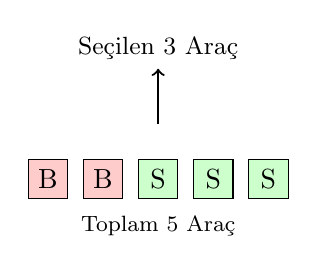
\begin{tikzpicture}[scale=0.7]
                \foreach \i in {1,2} \node[draw, fill=red!20, minimum size=0.5cm] at (\i, 1) {B};
                \foreach \i in {3,4,5} \node[draw, fill=green!20, minimum size=0.5cm] at (\i, 1) {S};
                \node[below] at (3,0.5) {\footnotesize Toplam 5 Araç};
                \draw[->, thick] (3, 2) -- (3, 3) node[above] {\small Seçilen 3 Araç};
            \end{tikzpicture}
        \end{column}
    \end{columns}

    \vspace{0.4cm}
    \begin{block}{Görevimiz}
        \begin{enumerate}
            \item[(a)] Tüm olası sonuçları içeren \textbf{Örnek Uzayı ($S$)} listeleyiniz.
            \item[(b)] Her sonuç için $X$ rastgele değişkeninin değerini bulunuz.
            \item[(c)] $\{X = 1\}$ olayını (tam bir aracın boyalı olması) küme olarak yazınız.
        \end{enumerate}
    \end{block}
\end{frame}



\begin{frame}{Çözüm: Araba Boyası Analizi}
    \setbeamercovered{transparent=7}
    \uncover<2->{
        \small
        {\color{red!80!black}
        \textbf{(a) Örnek Uzayı ($S$):} \\
        Seçilen 3 araçtaki renk kombinasyonlarını inceleriz ($B$: Boyalı, $S$: Sağlam). \\
        Toplamda \textbf{2 boyalı} ve \textbf{3 sağlam} aracımız var. Bu nedenle seçtiğimiz 3 aracın *hepsinin* boyalı olma ihtimali (BBB) **mümkün değildir.**
        \[
        S = \{BBS, BSB, SBB, BSS, SBS, SSB, SSS\}
        \]

        \vspace{0.1cm}
        \textbf{(b) Değişken Değerleri ($X$):} \\
        Rastgele değişkenimiz ``$X$'', içindeki $B$ harfi (boyalı araç) sayısını temsil eder. Her sonuç için $B$ harfini sayıyoruz:
        \begin{center}
        \begin{tabular}{rccccccc}
          \toprule
          Sonuç ($\omega$): & $BBS$ & $BSB$ & $SBB$ & $BSS$ & $SBS$ & $SSB$ & $SSS$ \\
          \midrule
          $X(\omega)$: & \textbf{2} & \textbf{2} & \textbf{2} & \textbf{1} & \textbf{1} & \textbf{1} & \textbf{0} \\
          \bottomrule
        \end{tabular}
        \end{center}

        \vspace{0.1cm}
        \textbf{(c) $\{X = 1\}$ Olayı:} \\
        İçinde \textbf{sadece ve tam olarak 1 tane $B$} olan durumları tablodan bulup seçiyoruz:
        \[
        \{X = 1\} = \{BSS, SBS, SSB\}
        \]
        }
    }
\end{frame}

\begin{frame}{Kavramsal Köprü: Torba Çekimi Örneği}
    Bir torbada 5 kırmızı ve 3 siyah top vardır. Yerine koymadan 2 top çekiliyor.
    \begin{itemize}
        \item $Y$: Çekilen kırmızı top sayısı.
    \end{itemize}

    \textbf{Sorular:}
    \begin{enumerate}
        \item[(a)] Örnek uzayı $S$ yazınız.
        \item[(b)] $Y$'nin her örnek nokta için aldığı değerleri tabloya dökünüz.
        \item[(c)] $\{Y \ge 1\}$ olayını örnek uzay cinsinden yazınız.
        \item[(d)] $Y$ ayrık mı, sürekli mi? Gerekçelendiriniz.
    \end{enumerate}
\end{frame}

\begin{frame}{Soru 3: Çözüm}
    \setbeamercovered{transparent=7}
    \uncover<2->{
        \small
        {\color{red}
        \textbf{(a) Örnek uzay:} 2 çekiliş için renk sonuçları (sıralı):
        \[
        S=\{KK, KS, SK, SS\}
        \]
        (\(K\): kırmızı, \(S\): siyah.)

        \vspace{0.1cm}
        \textbf{(b)} Her sonuç için \(Y\) (kırmızı sayısı):
        \begin{center}
        \begin{tabular}{ccccc}
          \toprule
          \(\omega\) & \(KK\) & \(KS\) & \(SK\) & \(SS\) \\
          \midrule
          \(Y(\omega)\) & 2 & 1 & 1 & 0 \\
          \bottomrule
        \end{tabular}
        \end{center}

        \vspace{0.1cm}
        \textbf{(c)} \(\{Y \ge 1\}=\{KK, KS, SK\}\).

        \vspace{0.1cm}
        \textbf{(d)} \(Y\) \textbf{ayrık}tır; çünkü alabileceği değerler kümesi sonludur:
        \[
        Y \in \{0,1,2\}.
        \]
        }
    }
\end{frame}




% ===================================================================
% BÖLÜM 3: AYRIK OLASILIK DAĞILIMI (Kitap 3.2)
% ===================================================================
\section{Ayrık Olasılık Dağılımı (Bölüm 3.2)}
\subsection{Olasılık Kütle Fonksiyonu (PMF: Probability Mass Function) Tanımı ve Özellikleri}

\begin{frame}{Olasılık Kütle Fonksiyonu (PMF: Probability Mass Function) Nedir?}
\begin{block}{Tanım 3.4 (Kitap): Olasılık Fonksiyonu}
  Ayrık rastgele değişken $X$'in olasılık fonksiyonu $f(x) = P(X = x)$ şu koşulları sağlar:
  \begin{enumerate}
    \item $f(x) \ge 0$ \quad (her değer için; yani olasılık negatif olamaz, en az 0'dır).
    \item $\displaystyle\sum_{x} f(x) = 1$ \quad (tüm olası değerlerin olasılıkları toplanınca sonuç mutlaka 1 olur).
    \item $P(X = x) = f(x)$ \quad (belirli bir $x$ değerinin olasılığı, PMF'nin o noktadaki değeridir).
  \end{enumerate}
\end{block}

\begin{exampleblock}{Ne demek?}
  PMF (Olasılık Kütle Fonksiyonu, Probability Mass Function), her olası $x$ değerine bir olasılık atayan tablodur.
  Tüm olasılıklar toplamı tam olarak~1 etmelidir.
\end{exampleblock}
\end{frame}


\begin{frame}{Örnek 3.8 (Kitaptan): Dizüstü Bilgisayar Satışı}
\footnotesize
\begin{columns}[T]
  \begin{column}{0.55\textwidth}
\begin{block}{Senaryo}
  Bir şirketten okula gönderilen \textbf{20 dizüstü bilgisayardan 3 tanesi arızalıdır},
  geri kalan \textbf{17 tanesi ise sağlamdır}. Okul bu kutudan
  \textbf{rastgele 2 bilgisayar} seçerek satın alıyor.
  
  \vspace{0.15cm}
  Değişken: $X =$ Alınan 2 bilgisayar arasındaki \textbf{arızalı bilgisayar sayısı}.
\end{block}

    \begin{block}{$X$ Değişkeninin Olasılık Dağılımı (PMF)}
      \centering
      \begin{tabular}{cc}
        \toprule
        $x$ & $f(x)$ \\
        \midrule
        0 & $136/190 \approx 0.716$ \\
        1 & $51/190 \approx 0.268$ \\
        2 & $3/190 \approx 0.016$ \\
        \bottomrule
      \end{tabular}
    \end{block}

  \end{column}
  \begin{column}{0.40\textwidth}
    \begin{alertblock}{Çözüm}
      $X \in \{0, 1, 2\}$. Kombinasyon mantığı ile:
      \[
      f(0) = \frac{\binom{3}{0}\binom{17}{2}}{\binom{20}{2}} = \frac{136}{190}
      \]
      \[
      f(1) = \frac{\binom{3}{1}\binom{17}{1}}{\binom{20}{2}} = \frac{51}{190}
      \]
      \[
      f(2) = \frac{\binom{3}{2}\binom{17}{0}}{\binom{20}{2}} = \frac{3}{190}
      \]
    \end{alertblock}

    \begin{block}{Kontrol}
      \[
      \frac{136}{190} + \frac{51}{190} + \frac{3}{190} = \frac{190}{190} = 1 \;\checkmark
      \]
    \end{block}
  \end{column}
\end{columns}
\end{frame}

\begin{frame}{Örnek 3.9 (Kitaptan): Hava Yastığı Satışı}
\footnotesize
\begin{columns}[T]
  \begin{column}{0.55\textwidth}
    \begin{block}{Senaryo ve Soru}
      Bir acentada her satışta hava yastıklı araç satılma olasılığı \%50'dir.
      Birbirinden bağımsız sıradaki 4 satış için
      $X$: hava yastıklı satılan araç sayısı olsun.
      $X$'in olasılık fonksiyonunu (PMF) bulunuz.
    \end{block}

    \begin{block}{PMF Tablosu}
      \centering
      \begin{tabular}{cc}
        \toprule
        $x$ & $f(x)$ \\
        \midrule
        0 & $1/16$ \\
        1 & $4/16 = 1/4$ \\
        2 & $6/16 = 3/8$ \\
        3 & $4/16 = 1/4$ \\
        4 & $1/16$ \\
        \bottomrule
      \end{tabular}
    \end{block}
  \end{column}
  \begin{column}{0.40\textwidth}
    \begin{alertblock}{Çözüm ve Açıklama}
      \textbf{Adım 1: Tüm olası durumlar sayısı}\\
      Her bir satıştaki aracın hava yastıklı olup olmaması (Evet/Hayır) bağımsızdır. $2 \times 2 \times 2 \times 2 = 16$ farklı satış senaryosu doğar.

      \textbf{Adım 2: Formülün Mantığı ($f(x)$)}\\
      4 araç içerisinden tam olarak $x$ tanesinin hava yastıklı olma kombinasyonu $\binom{4}{x}$'tir. Her bir durumun olasılığı eşit olduğundan, toplam olasılık $\frac{\binom{4}{x}}{16}$ şeklinde ifade edilir.
      \[
      f(x) = \frac{\binom{4}{x}}{16}, \quad x \in \{0, 1, 2, 3, 4\}
      \]
      Örneğin; 2 aracın hava yastıklı olması $f(2) = \frac{\binom{4}{2}}{16} = \frac{6}{16} = \frac{3}{8}$ olur.
    \end{alertblock}
    \begin{block}{Kontrol ve Gözlem}
      \[
      \sum_{x=0}^{4} f(x)=1 \;\checkmark
      \]
      Dağılım simetriktir: $f(0)=f(4)$ ve $f(1)=f(3)$.
    \end{block}
  \end{column}
\end{columns}
\end{frame}

\begin{frame}{Olasılık Dağılımının Görselleştirilmesi (Örnek 3.9)}
    Kesikli bir rastgele değişkenin olasılık kütle fonksiyonu (PMF) görselleştirilirken genellikle \textbf{çubuk grafiği} kullanılır. Bu gösterimde:
    
    \begin{itemize}
        \item \textbf{Yatay Eksen ($x$):} Rastgele değişkenin alabileceği değerleri gösterir.
        \item \textbf{Dikey Eksen ($f(x)$):} Her çubuğun yüksekliği, doğrudan o değerin teorik gerçekleşme olasılığına ($P(X=x)$) eşittir.
    \end{itemize}

    \begin{center}
        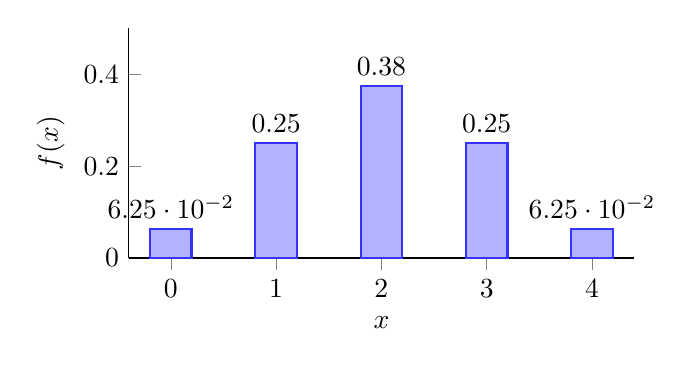
\begin{tikzpicture}
            \begin{axis}[
                ybar,
                bar width=15pt,
                symbolic x coords={0,1,2,3,4},
                xtick=data,
                nodes near coords,
                nodes near coords align={vertical},
                ymin=0, ymax=0.5,
                width=8cm, height=4.5cm,
                axis lines*=left,
                ylabel={$f(x)$},
                xlabel={$x$}
            ]
                \addplot[fill=blue!30, draw=blue!80, thick] coordinates {(0,0.0625) (1,0.25) (2,0.375) (3,0.25) (4,0.0625)};
            \end{axis}
        \end{tikzpicture}
    \end{center}
    
    \vspace{-0.4cm}
    \begin{center}
        \scriptsize \textit{Not: Bu tür dağılım grafiklerinde, grafikteki tüm çubukların yükseklikleri toplamı daima 1'e eşittir ($\sum f(x) = 1$).}
    \end{center}
\end{frame}



\subsection{Birikimli Dağılım Fonksiyonu (CDF: Cumulative Distribution Function)}

\begin{frame}{Birikimli Dağılım Fonksiyonu (CDF: Cumulative Distribution Function)}
    \small
    \begin{block}{Tanım 3.5: Birikimli Dağılım Fonksiyonu (CDF)}
        Büyük $F$ harfi ile gösterilen bu fonksiyon, bir rastgele değişkenin ($X$), belirli bir $x$ değerine \textbf{eşit veya daha küçük} olma olasılıklarının \textbf{toplamını (birikimini)} ifade eder:
        \[
        F(x) = P(X \le x) = \sum_{t \le x} f(t), \qquad -\infty < x < \infty.
        \]
    \end{block}

    \begin{exampleblock}{Nasıl Düşünmeliyiz? (Kavramsal Bakış)}
        \begin{itemize}
            \item \textbf{Kumbara Mantığı:} PMF ($f(x)$) sadece ``tam o x noktasındaki'' ihtimali bize söylerken; CDF ($F(x)$) en baştan başlayarak istenilen $x$ noktasına kadar gelen \textbf{tüm olasılıkları üst üste ekleyerek} ilerler.
            \item \textbf{Hiç Azalmaz:} $F(x)$, sürekli eski olasılıkların üzerine yeni değerler ekleyerek ilerler. Bu nedenle grafik yukarı doğru giderek artan bir \textbf{basamak fonksiyonu} (merdiven) şeklindedir ve en sonda mutlak suretle toplam olasılık olan \textbf{1'e} ulaşır.
            \item \textbf{Kümülatif Sıçramalar:} Grafikte yaşanan her yukarı yönlü  sıçrama miktarı, tam o noktadaki $f(x)$ (tekil olasılık) değerinin ta kendisidir. Toplam birikimden bir önceki basamağı çıkararak güncel ihtimali bulabiliriz: $f(x) = F(x) - F(x^{-})$.
        \end{itemize}
    \end{exampleblock}
\end{frame}

\begin{frame}{Uygulama: CDF Hesaplama (Örnek 3.10 - Bölüm 1)}
    \footnotesize
    \begin{block}{Senaryo (Hava Yastığı Problemi)}
      Bir acentada her satışta hava yastıklı araç satılma olasılığı \%50'dir. Sıradaki \textbf{4 satış} için $X$, hava yastıklı satılan araç sayısı olsun.
      Bu olayın tekil olasılıkları (PMF) şöyledir:
      \[
      f(0)=\frac{1}{16}, \; f(1)=\frac{4}{16}, \; f(2)=\frac{6}{16}, \; f(3)=\frac{4}{16}, \; f(4)=\frac{1}{16}
      \]
      \textbf{Görev:} Bu dağılımın Birikimli Dağılım Fonksiyonunu (CDF) adım adım oluşturalım. Daha sonra $f(2) = 3/8$ olduğunu doğrulamak için birikimli mantığı kullanalım.
    \end{block}
    
    \begin{exampleblock}{Adım Adım Birikim (CDF Yapımı)}
      Kumbara mantığıyla her $x$ seviyesinde bir önceki olasılıkları da üst üste ekliyoruz:
      \vspace{0.1cm}
      \begin{columns}[T]
          \begin{column}{0.48\textwidth}
              \begin{itemize}
                  \item $F(0) = f(0) = \frac{1}{16}$
                  \item $F(1) = F(0) + f(1) = \frac{1}{16} + \frac{4}{16} = \frac{5}{16}$
                  \item $F(2) = F(1) + f(2) = \frac{5}{16} + \frac{6}{16} = \frac{11}{16}$
              \end{itemize}
          \end{column}
          \begin{column}{0.48\textwidth}
              \begin{itemize}
                  \item $F(3) = F(2) + f(3) = \frac{11}{16} + \frac{4}{16} = \frac{15}{16}$
                  \item $F(4) = F(3) + f(4) = \frac{15}{16} + \frac{1}{16} = \mathbf{1} \;\checkmark$
              \end{itemize}
          \end{column}
      \end{columns}
      \vspace{0.1cm}
    \end{exampleblock}
\end{frame}

\begin{frame}{Uygulama: CDF Grafiği ve Doğrulama (Bölüm 2)}
    \footnotesize
    \begin{columns}[T]
        \begin{column}{0.48\textwidth}
            \begin{block}{Doğrulama (Geriye Dönüş)}
              Sadece 2 olma ihtimalini (tekil olasılık), 2 noktasına kadarki \textbf{toplam} birikimden, 1 noktasına kadarki birikimi çıkararak bulabiliriz:
              \[
              f(2) = F(2) - F(1) = \frac{11}{16} - \frac{5}{16} = \frac{6}{16} = \mathbf{\frac{3}{8}} \;\checkmark
              \]
            \end{block}
            
            \vspace{0.3cm}
            \begin{exampleblock}{Grafiğin İncelenmesi}
                \begin{itemize}
                    \item \textbf{Asla Düşmez:} Eski değerler kumbarada kaldığı için çizgi hiçbir zaman aşağı inmez.
                    \item \textbf{Sıçrama Miktarı:} Grafikteki herhangi bir dikey sıçramanın (boyunun) miktarı, fonksiyonun tam o noktadaki $f(x)$ ihtimaline eşittir.
                \end{itemize}
            \end{exampleblock}
        \end{column}
        
        \begin{column}{0.48\textwidth}
            \centering
            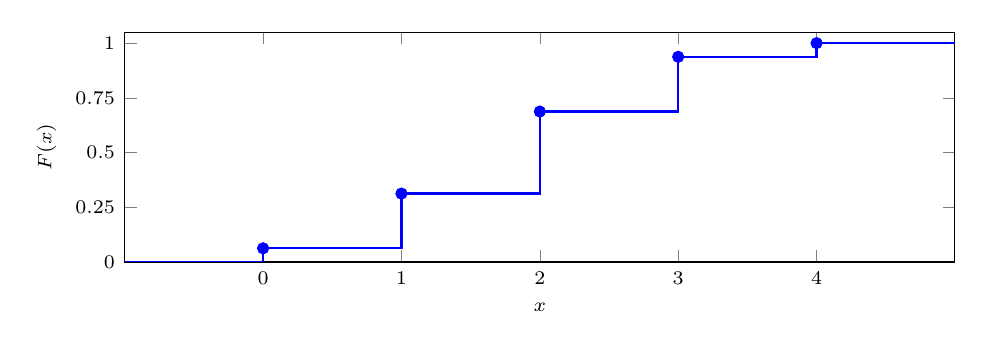
\begin{tikzpicture}
              \begin{axis}[
                width=\linewidth,
                height=4.5cm,
                xmin=-1, xmax=5,
                ymin=0, ymax=1.05,
                xtick={0,1,2,3,4},
                ytick={0,0.25,0.5,0.75,1},
                tick label style={font=\scriptsize},
                label style={font=\scriptsize},
                xlabel={$x$}, ylabel={$F(x)$}
              ]
                \addplot[thick, blue, const plot] coordinates {
                  (-1,0) (0,0.0625) (1,0.3125) (2,0.6875) (3,0.9375) (4,1) (5,1)
                };
                \addplot[only marks, blue, mark=*] coordinates {
                    (0,0.0625) (1,0.3125) (2,0.6875) (3,0.9375) (4,1)
                };
              \end{axis}
            \end{tikzpicture}
        \end{column}
    \end{columns}
\end{frame}

\subsection{Pekiştirme Soruları}

\begin{frame}{Soru 2: Televizyon Setleri}
    7 televizyonluk bir sevkiyatta 2'si arızalıdır. Bir otel rastgele 3 televizyon satın alıyor.

    $X$: arızalı televizyon sayısı.

    \textbf{Sorular:}
    \begin{enumerate}
        \item[(a)] $X$'in olasılık dağılımını (PMF tablosunu) bulunuz.
        \item[(b)] PMF'nin geçerli olduğunu ($\sum f(x) = 1$) doğrulayınız.
        \item[(c)] CDF'yi $F(x)$ biçiminde yazınız ve $P(X \ge 1)$ hesaplayınız.
    \end{enumerate}
\end{frame}

\begin{frame}{Soru 2: Çözüm}
    \setbeamercovered{transparent=7}
    \uncover<2->{
    \normalsize
    {\color{red}
    \textbf{(a) PMF:} $X \in \{0,1,2\}$ ve
    \[
    f(x)=\frac{\binom{2}{x}\binom{5}{3-x}}{\binom{7}{3}}
    \]
    \[
    f(0)=\frac{10}{35}=\frac{2}{7},\quad
    f(1)=\frac{20}{35}=\frac{4}{7},\quad
    f(2)=\frac{5}{35}=\frac{1}{7}
    \]

    \textbf{(b) Kontrol:}
    \[
    \frac{2}{7}+\frac{4}{7}+\frac{1}{7}=1 \;\checkmark
    \]

    \textbf{(c) CDF ve istenen olasılık:}
    \[
    F(0)=\frac{2}{7},\qquad
    F(1)=\frac{6}{7},\qquad
    F(2)=1
    \]
    \[
    P(X\ge1)=1-F(0)=1-\frac{2}{7}=\frac{5}{7}\approx0.714
    \]
    }
    }
\end{frame}



\begin{frame}{Hesaplamayı Hızlandırmak: CDF ile Aralık Olasılığı}
    $F(x)$ biliniyorsa, $X$'in belli bir aralıkta olma olasılığı kolayca bulunur:

    \begin{block}{Formül}
        \[
        P(a < X \le b) = F(b) - F(a)
        \]
    \end{block}

    \textbf{İspat mantığı:}
    \[
    \{X \le b\} = \{X \le a\} \cup \{a < X \le b\}
    \]
    \[
    F(b) = F(a) + P(a < X \le b)
    \]

    \textbf{Ayrıca:} Ayrık değişkenlerde PMF'ye geri dönmek için:
    $f(x) = F(x) - F(x^{-})$
    \scriptsize \textit{(Eğer değerler tam sayı ise $f(x)=F(x)-F(x-1)$ pratik olarak kullanılabilir.)}
\end{frame}

% ===================================================================
% BÖLÜM 4: SÜREKLİ OLASILIK DAĞILIMI (Kitap 3.3)
% ===================================================================
\section{Sürekli Olasılık Dağılımı}
\subsection{Olasılık Yoğunluk Fonksiyonu (PDF)}

\begin{frame}{Kavrama Giriş: Olasılık Yoğunluk Fonksiyonu (PDF: Probability Density Function)}
\begin{block}{Tanım: Olasılık Yoğunluk Fonksiyonu}
  Sürekli $X$ için $f(x)$ bir PDF'dir, eğer:
  \begin{enumerate}
    \item $f(x) \ge 0$ \quad (her $x$ için).
    \item $\displaystyle\int_{-\infty}^{\infty} f(x)\,dx = 1$ \quad (toplam alan 1).
    \item $\displaystyle P(a < X < b) = \int_{a}^{b} f(x)\,dx$ \quad (olasılık = alan).
  \end{enumerate}
\end{block}

\begin{alertblock}{Önemli Fark: Neden İntegral Kullanıyoruz?}
  Ayrık değişkenlerde (PMF) olasılıklar tekil olarak formülden çıkıp \textbf{toplanırken} ($\sum$), sürekli değişkenlerde aralarda sonsuz ondalıklı nokta olduğu için $f(x)$ tek başına olasılık değil \textbf{yoğunluk} belirtir. Kümülatif toplama işini ise artık \textbf{integral (alan hesabı)} devralır.
\end{alertblock}
\end{frame}

\begin{frame}{Alanları Olasılığa Dönüştürmek: Sıcaklık Hatası}
\footnotesize
\begin{columns}[T]
  \begin{column}{0.55\textwidth}
    \begin{block}{Problem}
      Kontrollü bir deneyde sıcaklık hatası ($^\circ$C):
      \[
      f(x) =
      \begin{cases}
        \dfrac{x^2}{3}, & -1 < x < 2,\\[4pt]
        0, & \text{diğer}.
      \end{cases}
      \]
      (a) $f(x)$'in geçerli bir PDF olduğunu doğrulayın.\\
      (b) $P(0 < X \le 1)$ hesaplayın.
    \end{block}
  \end{column}
  \begin{column}{0.42\textwidth}
    \begin{alertblock}{Çözüm}
      \textbf{(a)} $f(x) \ge 0$ açık. Toplam alan:
      \[
      \int_{-1}^{2} \frac{x^2}{3}\,dx = \frac{x^3}{9}\bigg|_{-1}^{2} = \frac{8}{9} + \frac{1}{9} = 1 \;\checkmark
      \]

      \textbf{(b)}
      \[
      P(0 < X \le 1) = \int_{0}^{1} \frac{x^2}{3}\,dx = \frac{x^3}{9}\bigg|_{0}^{1} = \frac{1}{9}
      \]
      \[
      \boxed{P(0 < X \le 1) = 1/9 \approx 0.111}
      \]
    \end{alertblock}
  \end{column}
\end{columns}
\end{frame}

\subsection{Sürekli Birikimli Dağılım Fonksiyonu (CDF: Cumulative Distribution Function)}

\begin{frame}{Sürekli Birikimli Dağılım Fonksiyonu (CDF) ve Kullanımı}
\begin{block}{Tanım 3.7: Sürekli Birikimli Dağılım Fonksiyonu (CDF)}
  Sürekli bir rastgele değişken $X$'in olasılık yoğunluk fonksiyonu $f(x)$ ise, Kümülatif (Birikimli) Dağılım Fonksiyonu $F(x)$ şu şekildedir:
  \[
  F(x) = P(X \le x) = \int_{-\infty}^{x} f(t)\,dt, \qquad -\infty < x < \infty.
  \]
\end{block}

\begin{block}{Tanım 3.7'nin Bir Sonucu Olarak:}
  \begin{enumerate}
    \item $P(a < X < b) = F(b) - F(a)$
    \item \textbf{Eğer türev mevcutsa,} $f(x) = \frac{dF(x)}{dx}$
  \end{enumerate}
\end{block}
\end{frame}

\begin{frame}{Pratik Bir Yaklaşım: CDF'den Olasılık Hesabı}
\footnotesize
\begin{columns}[T]
  \begin{column}{0.55\textwidth}
    \begin{block}{Problem}
      Örnek 3.11'deki PDF için $F(x)$'i bulun ve $P(0 < X \le 1)$'i doğrulayın.
    \end{block}
    \begin{alertblock}{Çözüm}
      $-1 < x < 2$ için:
      \[
      F(x) = \int_{-1}^{x} \frac{t^2}{3}\,dt = \frac{x^3 + 1}{9}
      \]
      Tam tanım:
      \[
      F(x) =
      \begin{cases}
        0, & x < -1,\\
        \frac{x^3+1}{9}, & -1 \le x < 2,\\
        1, & x \ge 2.
      \end{cases}
      \]
    \end{alertblock}
  \end{column}
  \begin{column}{0.42\textwidth}
    \begin{block}{Doğrulama}
      \[
      P(0 < X \le 1) = F(1) - F(0)
      \]
      \[
      = \frac{1+1}{9} - \frac{0+1}{9} = \frac{2}{9} - \frac{1}{9} = \frac{1}{9} \;\checkmark
      \]
    \end{block}
    \centering
    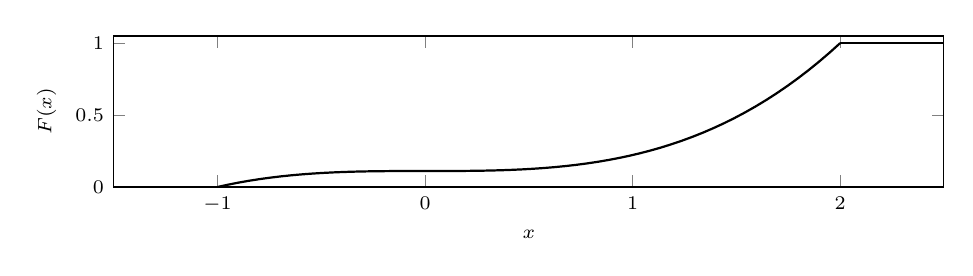
\begin{tikzpicture}
      \begin{axis}[
        width=\linewidth,
        height=3.5cm,
        xmin=-1.5, xmax=2.5,
        ymin=0, ymax=1.05,
        xtick={-1,0,1,2},
        ytick={0,0.5,1.0},
        tick label style={font=\scriptsize},
        label style={font=\scriptsize},
        xlabel={$x$}, ylabel={$F(x)$}
      ]
        \addplot[thick, domain=-1:2, samples=60] {(x^3+1)/9};
        \addplot[thick, domain=-1.5:-1] {0};
        \addplot[thick, domain=2:2.5] {1};
      \end{axis}
    \end{tikzpicture}
  \end{column}
\end{columns}
\end{frame}

\subsection{Pekiştirme Soruları}

\begin{frame}{Soru 3: Elektrik Süpürgesi}
    Bir ailenin yılda elektrik süpürgesini çalıştırma süresi (100 saat biriminde) $X$ ile modelleniyor:
    \[
    f(x) =
    \begin{cases}
      x, & 0 < x < 1,\\
      2 - x, & 1 \le x < 2,\\
      0, & \text{diğer}.
    \end{cases}
    \]
    \begin{center}
      \scriptsize \textit{(Not: Sürekli sınırlardaki eşittir ($\le$) işareti, noktasal probability 0 olduğu için integrasyondaki alana hiçbir etki etmez.)}
    \end{center}

    \textbf{Sorular:}
    \begin{enumerate}
      \item[(a)] $f(x)$'in geçerli PDF olduğunu doğrulayınız.
      \item[(b)] Yılda 120 saatten az kullanma olasılığını bulunuz ($P(X < 1.2)$).
    \end{enumerate}
\end{frame}

\begin{frame}{Soru 3: Çözüm}
    \setbeamercovered{transparent=7}
    \uncover<2->{
    \normalsize
    {\color{red}
    \textbf{(a) PDF kontrolü:}
    \[
    \int_{0}^{1} x\,dx + \int_{1}^{2} (2-x)\,dx
    = \frac{1}{2} + \frac{1}{2} = 1 \;\checkmark
    \]

    \textbf{(b) Olasılık hesabı:}
    \[
    P(X < 1.2)
    = \int_{0}^{1} x\,dx + \int_{1}^{1.2} (2-x)\,dx
    = 0.5 + 0.18 = 0.68
    \]

    $\boxed{P(X < 1.2) = 0.68 = \%68}$
    }
    }
\end{frame}



% ===================================================================
% BÖLÜM 5: KAVRAMI TOPARLA
% ===================================================================
\section{Kavramsal Özet ve Kapanış}
\subsection{PMF--PDF--CDF İlişkisi}

\begin{frame}{Büyük Resim: PMF, PDF ve CDF'nin Uyumlu Birlikteliği}
\footnotesize
\begin{columns}[T]
  \begin{column}{0.48\textwidth}
    \begin{block}{Ayrık Değişken}
      \begin{itemize}
        \item $f(x) = P(X = x)$ \quad (PMF)
        \item $F(x) = \sum_{t \le x} f(t)$ \quad (toplam)
        \item $f(x) = F(x) - F(x^{-})$ \quad (basamak farkı)
      \end{itemize}
    \end{block}
  \end{column}
  \begin{column}{0.48\textwidth}
    \begin{block}{Sürekli Değişken}
      \begin{itemize}
        \item $f(x)$ yoğunluktur \quad (PDF)
        \item $F(x) = \int_{-\infty}^{x} f(t)\,dt$ \quad (integral)
        \item $f(x) = F'(x)$ \quad (türev)
      \end{itemize}
    \end{block}
  \end{column}
\end{columns}

\vspace{0.3cm}
\centering
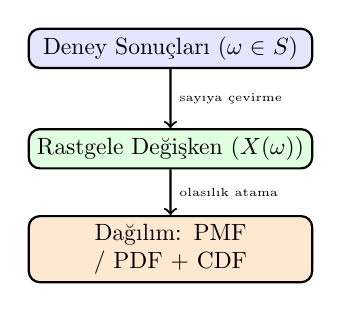
\begin{tikzpicture}[node distance=1.5cm, auto, thick, scale=0.85, transform shape]
  \node (P1) [draw, rounded corners, fill=blue!10, text width=4cm, align=center]
  {Deney Sonuçları ($\omega \in S$)};
  \node (P2) [draw, rounded corners, fill=green!12, below of=P1, text width=4cm, align=center]
  {Rastgele Değişken ($X(\omega)$)};
  \node (P3) [draw, rounded corners, fill=orange!18, below of=P2, text width=4cm, align=center]
  {Dağılım: PMF / PDF + CDF};

  \draw[->] (P1) -- (P2) node[midway,right,font=\tiny] {sayıya çevirme};
  \draw[->] (P2) -- (P3) node[midway,right,font=\tiny] {olasılık atama};
\end{tikzpicture}
\end{frame}

\begin{frame}[fragile]{Zihinsel Antrenman: Doğru Kavramı Seçin}
    \begin{itemize}[<+->]
        \item ``5 ürün arasındaki kusurlu sayısı'' $\Rightarrow$ \textbf{Ayrık} (sayım)
        \item ``Makinenin ömrü kaç saat?'' $\Rightarrow$ \textbf{Sürekli} (ölçüm)
        \item ``Her bir noktasal durum için $P(X = x) = 0$ olan değişken türü?'' $\Rightarrow$ \textbf{Sürekli}
        \item ``$f(x) = P(X = x)$ formülünün adı?'' $\Rightarrow$ \textbf{PMF}
        \item ``$\omega = SSA$ ise $X(\omega) = ?$'' ($X = \#A$) $\Rightarrow$ $X = 1$
        \item ``$F(2) - F(1) = ?$'' $\Rightarrow$ $P(1 < X \le 2)$
    \end{itemize}
\end{frame}

\begin{frame}{Kapanış Çıktısı: 3 Satırda Bu Hafta}
    \begin{block}{Refleksiyon}
        \begin{enumerate}
            \item Rastgele değişken bir \textbf{fonksiyon}dur; sonuçları sayılara çevirir ($X: S \to \mathbb{R}$).
            \item \textbf{Ayrık} $=$ sayım verisi (PMF ile), \textbf{Sürekli} $=$ ölçüm verisi (PDF ile).
            \item CDF, hem ayrık hem sürekli değişkenler için $F(x) = P(X \le x)$ biçiminde tanımlanır.
        \end{enumerate}
    \end{block}

    \vspace{0.3cm}
    \centering
    \textit{Haftaya: Beklenen Değer $E(X)$, Varyans $\mathrm{Var}(X)$ ve Ortak Dağılımlar.}
\end{frame}

% ===================================================================
% KAYNAKLAR VE APPENDIX
% ===================================================================
\section{Kaynaklar}
\begin{frame}[allowframebreaks]{Kaynaklar}
    \nocite{*}
    \printbibliography{}
\end{frame}

\appendix
\section{Yapay Zeka Asistanı}
\begin{frame}{Yapay Zeka Asistanınız: NotebookLM}
    \begin{columns}[T]
        \begin{column}{0.48\textwidth}
            \justifying{}
            \textbf{Ders Materyalleri ile Etkileşime Geçin!}

            Bu dersin tüm içeriği (sunumlar, makaleler ve notlar), Google'ın gelişmiş yapay zeka asistanı \textbf{NotebookLM} sistemine yüklenmiştir.

            \vspace{1em}
            \begin{itemize}
                \item \textbf{Anında Cevaplar:} Aklınıza takılanları sorun.
                \item \textbf{Özetler:} Karmaşık konuları basitçe öğrenin.
                \item \textbf{Audio Overview:} Dersi bir podcast gibi dinleyin.
            \end{itemize}

            \vspace{1.5em}
            \begin{center}
                {\setbeamercolor{button}{bg=red,fg=black}
                \href{https://notebooklm.google.com/notebook/37796201-25fd-4d44-aa3c-b673ce22f7a4}{\beamerbutton{\rule[-4ex]{0pt}{11ex}\Large \textbf{Hemen Deneyin}}}}
            \end{center}
        \end{column}

        \begin{column}{0.48\textwidth}
            \centering
            \includegraphics[width=\textwidth, height=0.6\textheight, keepaspectratio]{figures/notebooklm.jpg}
        \end{column}
    \end{columns}
\end{frame}

\begin{frame}[plain,noframenumbering]
    \begin{tikzpicture}[remember picture,overlay]
        \node[anchor=center, at=(current page.center), inner sep=0pt] {
            \includegraphics[width=\paperwidth, height=\paperheight]{figures/combined_qrs.png}
        };
        \node[anchor=south, at=(current page.south), yshift=0.5cm, fill=white!95, rounded corners, inner sep=10pt, text width=0.95\paperwidth, align=center] {
            \Large \textbf{\textcolor{blue}{Bizi Takip Edin!}} \\
            \vspace{0.3em}
            \small Ders tekrarlarıyla konuları pekiştirmek (YouTube), profesyonel proje ağlarına katılmak (LinkedIn) ve kampüs duyurularından anında haberdar olmak (Instagram) için topluluğumuza katılın.
        };
    \end{tikzpicture}
\end{frame}

\end{document}
